\section{i* modeling} \label{sec:Appendix1}


\section*{i{*} modeling}

The i{*} framework was developed for modelling and reasoning about
organizational environments and their information systems {[}2{]}.
It consists of two main modelling components. TheStrategic Dependency
(SD) model is used to describe the dependency relationships among
various actors in an organizational context. The Strategic Rationale
(SR) model is used to describe stakeholder interests and concerns,
and how they might be addressed by various configurations of systems
and environments {[}1{]}. We think that such a model can be a useful
instrument for requirement engineering because it is able to highlight
relationships between different levels of abstraction showing how
\emph{tasks} cooperates to fullfil \emph{goals} and how non functional
requirements (known ad \emph{soft goals} in the model) are affacted.
In this section we provide a simple model (Strategic Rationale model)
of a part of the TS system by using i{*} notation.

For further details and a exhaustive description of the notation refer
to:
\begin{lyxlist}{00.00.0000}
\item [{{[}1{]}}] E. Yu, Modelling Strategic Relationships for Process
Reengineering, Ph.D. thesis, also Tech. Report DKBS-TR- 94-6, Dept.
of Computer Science, University of Toronto, 1995.
\item [{{[}2{]}}] E. Yu `Towards Modelling and Reasoning Support for Early-Phase
Requirements Engineering' Proceedings of the 3rd IEEE Int. Symp. on
Requirements Engineering (RE'97) Jan. 6-8, 1997, Washington D.C.,
USA. pp. 226-235. 
\end{lyxlist}
\clearpage{}

\begin{landscape}

\begin{figure}
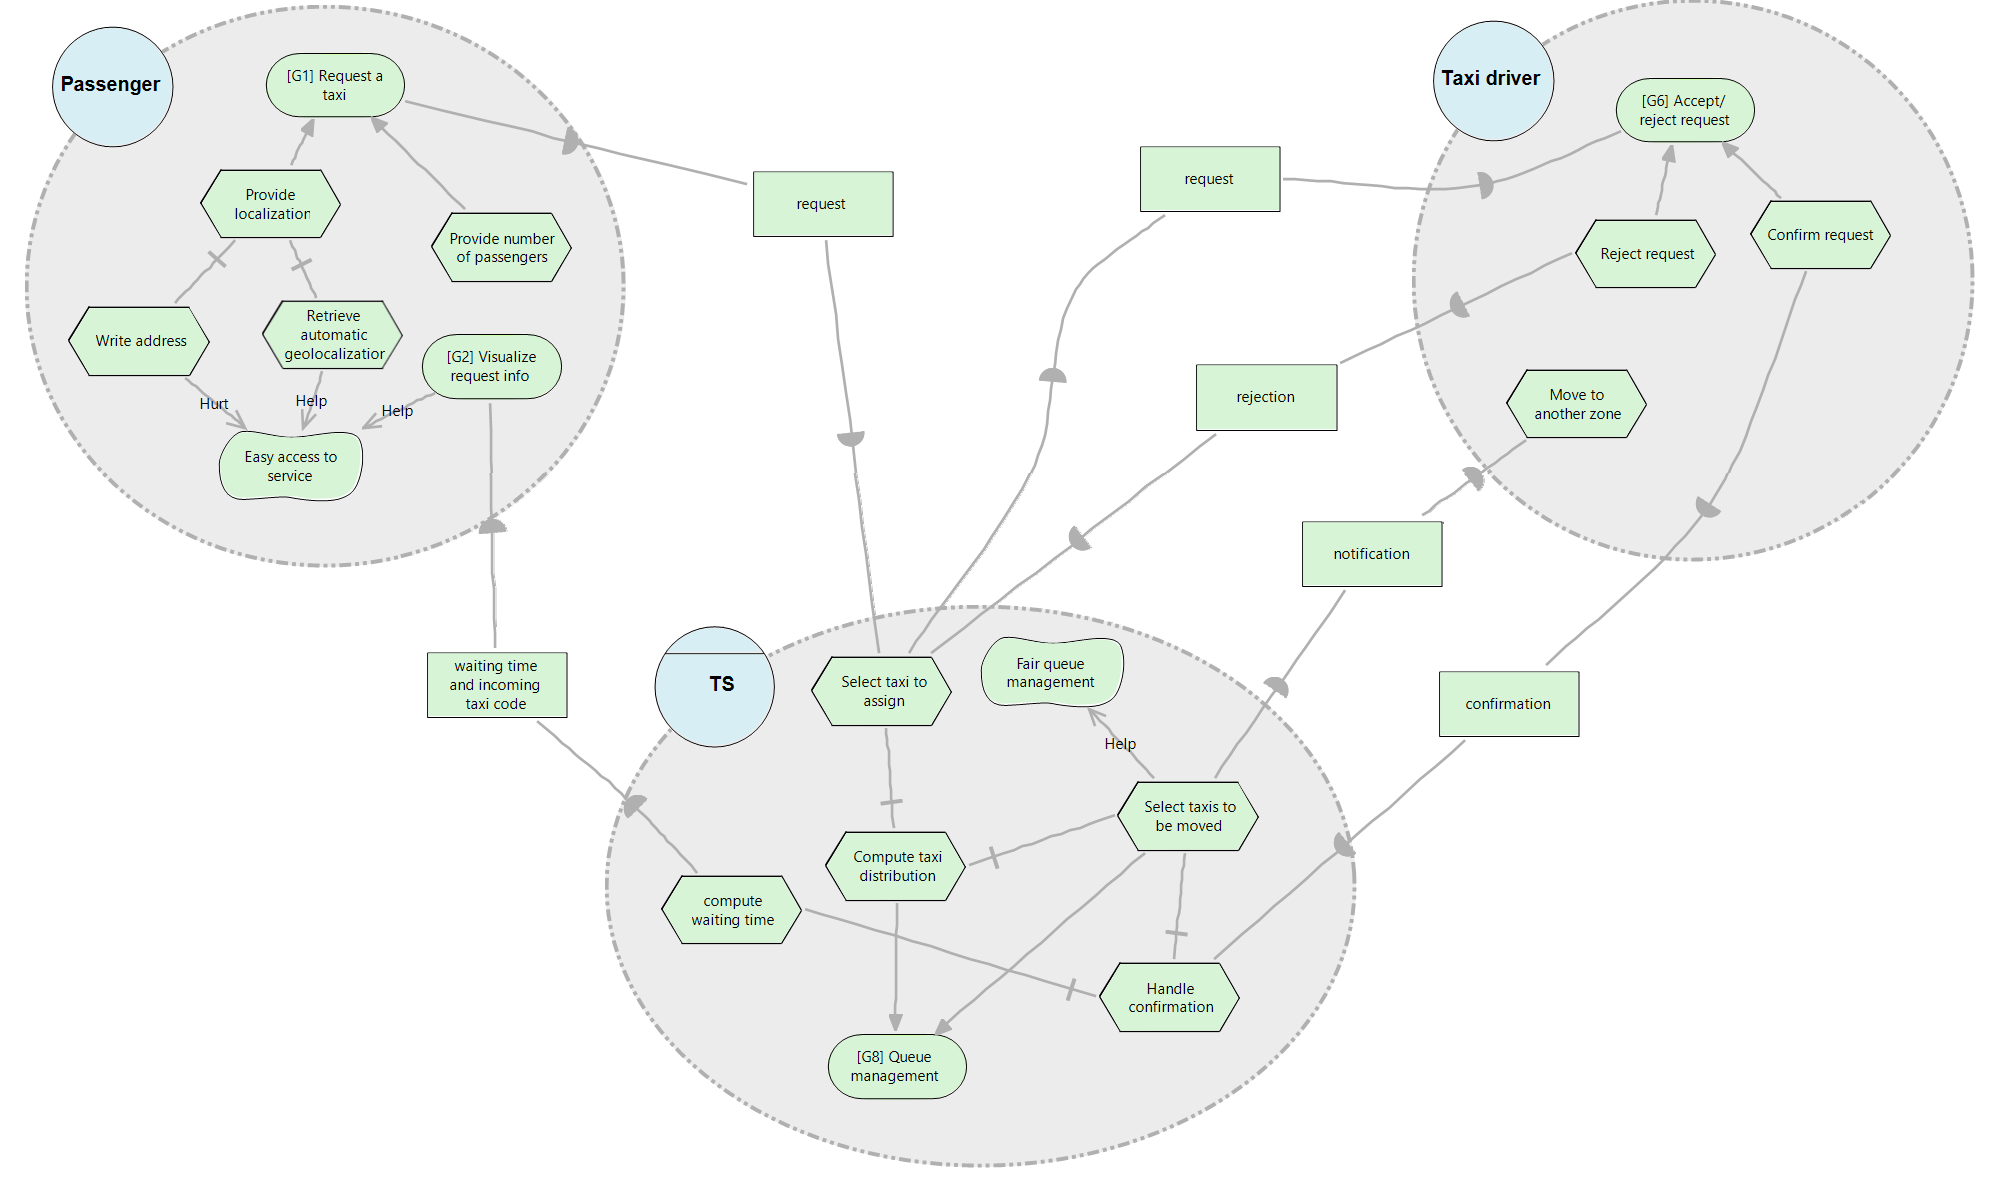
\includegraphics[scale=0.4]{appendix/istarmodeling}

\protect\caption{i{*} model}
\end{figure}


\end{landscape}

\clearpage{}

\section{Appendix} \label{sec:Appendix1}


\subsection*{Used tools}
\begin{enumerate}
\item \LyX{} visual editor for \LaTeX{} (\url{http://www.lyx.org/}) to
write this document.
\item Star UML \url{(http://staruml.io/}) for use case diagram, class diagram,
sequence diagram, activity diagram and state chart diagram.
\item Alloy Analyser 4.2 (\url{http://alloy.mit.edu/alloy/)} to build the
model and prove its consistency.
\item Balsamiq Mockup (\url{http://balsamiq.com/products/mockups/}) for
user inferface mockup generation.
\item OpenOME (\url{http://www.cs.toronto.edu/km/openome/OpenOME.html}),
an open-source requirements engineering tool for the i{*} model.
\end{enumerate}

\subsection*{Hours of works}

Time spent by each group member:
\begin{itemize}
\item Alberto Maria Metelli: 33 h
\item Riccardo Mologni: 33 h
\end{itemize}

\subsection*{Revision history}
\begin{lyxlist}{00.00.0000}
\item [{%
\begin{tabular}{>{\raggedright}p{1.5cm}|>{\raggedright}p{2cm}|>{\raggedright}p{3.5cm}|>{\raggedright}p{5cm}}
\hline 
\emph{Version} & \emph{Date} & \emph{Revision description} & \emph{Revision notes}\tabularnewline
\hline 
0.1 & 1-11-2015 & Initial draft & -\tabularnewline
\hline 
1.0 & 6-11-2015 & Final draft & -\tabularnewline
\hline 
\end{tabular}}]~\end{lyxlist}

